%Version 3.1 December 2024
% See section 11 of the User Manual for version history
%
%%%%%%%%%%%%%%%%%%%%%%%%%%%%%%%%%%%%%%%%%%%%%%%%%%%%%%%%%%%%%%%%%%%%%%
%%                                                                 %%
%% Please do not use \input{...} to include other tex files.       %%
%% Submit your LaTeX manuscript as one .tex document.              %%
%%                                                                 %%
%% All additional figures and files should be attached             %%
%% separately and not embedded in the \TeX\ document itself.       %%
%%                                                                 %%
%%%%%%%%%%%%%%%%%%%%%%%%%%%%%%%%%%%%%%%%%%%%%%%%%%%%%%%%%%%%%%%%%%%%%

%%\documentclass[referee,sn-basic]{sn-jnl}% referee option is meant for double line spacing

%%=======================================================%%
%% to print line numbers in the margin use lineno option %%
%%=======================================================%%

%%\documentclass[lineno,pdflatex,sn-basic]{sn-jnl}% Basic Springer Nature Reference Style/Chemistry Reference Style

%%=========================================================================================%%
%% the documentclass is set to pdflatex as default. You can delete it if not appropriate.  %%
%%=========================================================================================%%

%%\documentclass[sn-basic]{sn-jnl}% Basic Springer Nature Reference Style/Chemistry Reference Style

%%Note: the following reference styles support Namedate and Numbered referencing. By default the style follows the most common style. To switch between the options you can add or remove “Numbered” in the optional parenthesis. 
%%The option is available for: sn-basic.bst, sn-chicago.bst%  

%%\documentclass[pdflatex,sn-nature]{sn-jnl}% Style for submissions to Nature Portfolio journals
%%\documentclass[pdflatex,sn-basic]{sn-jnl}% Basic Springer Nature Reference Style/Chemistry Reference Style
\documentclass[pdflatex,sn-mathphys-num]{sn-jnl}% Math and Physical Sciences Numbered Reference Style
%%\documentclass[pdflatex,sn-mathphys-ay]{sn-jnl}% Math and Physical Sciences Author Year Reference Style
%%\documentclass[pdflatex,sn-aps]{sn-jnl}% American Physical Society (APS) Reference Style
%%\documentclass[pdflatex,sn-vancouver-num]{sn-jnl}% Vancouver Numbered Reference Style
%%\documentclass[pdflatex,sn-vancouver-ay]{sn-jnl}% Vancouver Author Year Reference Style
%%\documentclass[pdflatex,sn-apa]{sn-jnl}% APA Reference Style
%%\documentclass[pdflatex,sn-chicago]{sn-jnl}% Chicago-based Humanities Reference Style

%%%% Standard Packages
%%<additional latex packages if required can be included here>

\usepackage{graphicx}%
\usepackage{multirow}%
\usepackage{amsmath,amssymb,amsfonts}%
\usepackage{amsthm}%
\usepackage{mathrsfs}%
\usepackage[title]{appendix}%
\usepackage{xcolor}%
\usepackage{textcomp}%
\usepackage{manyfoot}%
\usepackage{booktabs}%
\usepackage{algorithm}%
\usepackage{algorithmicx}%
\usepackage{algpseudocode}%
\usepackage{listings}%
%%%%

%%%%%=============================================================================%%%%
%%%%  Remarks: This template is provided to aid authors with the preparation
%%%%  of original research articles intended for submission to journals published 
%%%%  by Springer Nature. The guidance has been prepared in partnership with 
%%%%  production teams to conform to Springer Nature technical requirements. 
%%%%  Editorial and presentation requirements differ among journal portfolios and 
%%%%  research disciplines. You may find sections in this template are irrelevant 
%%%%  to your work and are empowered to omit any such section if allowed by the 
%%%%  journal you intend to submit to. The submission guidelines and policies 
%%%%  of the journal take precedence. A detailed User Manual is available in the 
%%%%  template package for technical guidance.
%%%%%=============================================================================%%%%

%% as per the requirement new theorem styles can be included as shown below
\theoremstyle{thmstyleone}%
\newtheorem{theorem}{Theorem}%  meant for continuous numbers
%%\newtheorem{theorem}{Theorem}[section]% meant for sectionwise numbers
%% optional argument [theorem] produces theorem numbering sequence instead of independent numbers for Proposition
\newtheorem{proposition}[theorem]{Proposition}% 
%%\newtheorem{proposition}{Proposition}% to get separate numbers for theorem and proposition etc.

\theoremstyle{thmstyletwo}%
\newtheorem{example}{Example}%
\newtheorem{remark}{Remark}%

\theoremstyle{thmstylethree}%
\newtheorem{definition}{Definition}%

\raggedbottom
%%\unnumbered% uncomment this for unnumbered level heads

\tolerance=1
\emergencystretch=\maxdimen
\hyphenpenalty=10000
\hbadness=10000

\begin{document}
	
	\title[Article Title]{SecChaos-RL: A Threat-Aware Self-Adaptive Resilience Engineering Framework for Secure Software Systems}
	

	
\author*[1]{\fnm{Thurbilli } \sur{Karthik}}\email{405124053@nitt.edu}
\author[1]{\fnm{Michael   } \sur{Arock}}\email{michael@nitt.edu}
\author[2]{\fnm{Vinay} \sur{Raj}}\email{vinayraj@nitw.ac.in}

\affil[1]{\orgdiv{Department of Computer Applications}, \orgname{National Institute of Technology}, \orgaddress{ \city{Tiruchirappalli}, \postcode{620015}, \state{Tamil Nadu}, \country{India}}}
\affil[2]{\orgdiv{Department of Computational \& Data Science}, \orgname{National Institute of Technology}, \orgaddress{ \city{Warangal}, \postcode{506004}, \state{Telangana}, \country{India}}}


	
	%%==================================%%
	%% Sample for unstructured abstract %%
	%%==================================%%
	
	\abstract{Modern software systems are being deployed more and more as a distributed microservice architecture, increasing the attack surface and increasing the difficulty to be resilient to security threats and operational failures. Security Chaos Engineering (SCE) enhances the security resiliency by introducing intentional security issues, but the current practices of SCE are mostly static and manual. In this paper, we present a reinforcement learning (RL) framework for autonomous threat-aware mitigation in SCE environments (SecChaos-RL). The security mitigation process is represented as a Markov Decision Process (MDP), with which the agent learns adaptive mitigation policies based on an ongoing interaction with dynamically injected security faults. The proposed framework is compared with two state of the art algorithms, namely Deep Q-Network (DQN) and Advantage Actor-Critic (A2C), as well as Proximal Policy Optimization (PPO), in a simulated SCE environment with 30 independent random seeds. SecChaos-RL scores 88.95\% secure, which would take up 4.91\% of the simulated attack, service availability is maintained at 96.26\%, and the Mean Time to Recovery (MTTR) is reduced by 55.3\% from PPO. The findings suggest that adaptive reinforcement learning is able to achieve the balance between security, availability, and recovery, and shows its potential of autonomous mitigations to enhance software resilience in the security chaos scenario.}
	
	\keywords{Security Chaos Engineering, Software Resilience, Reinforcement Learning, Software Security, AI for Software Engineering, Adaptive Security}
	
	%%\pacs[JEL Classification]{D8, H51}
	
	%%\pacs[MSC Classification]{35A01, 65L10, 65L12, 65L20, 65L70}
	
	\maketitle
	
	\section{Introduction}
	Resilient digital ecosystems are crucial in critical infrastructure, healthcare, finance, and cloud computing, where software systems are growing quickly and fast~\cite{basiri2016chaos}. Distributed systems in the modern era are made up of hundreds of microservices, third party dependencies, and complex inter-service interactions that can be exploited by adversaries continuously \cite{myrbakken2020security}. Tools like static analysis, penetration testing, and vulnerability scanning are useful but do not provide a comprehensive understanding of system dynamics during an active security threat \cite{shortridge2023security}. The study of improving the detection of software vulnerabilities in recent years has focused on the learning of features by machine learning and representations at program levels \cite{tong2026osel}. 
	
	DevOps has revolutionized the way software is developed and delivered, with a focus on collaboration, automation, and continuous integration and deployment \cite{myrbakken2020security}. However, the speed and agility of DevOps practices could be affecting more traditional security controls and resulting in tension between speed and security assurance. It resulted in the creation of DevSecOps, the integration of security with DevOps. The integration is to make security part of the entire Software Development Life Cycle (SDLC) \cite{myrbakken2020security}. Security assessment for continuous deployment is still a big challenge in DevSecOps pipelines. Traditional security testing methods, such as vulnerability scanning, static application security testing (SAST) and dynamic application security testing (DAST) can provide information from a pre-production environment, but cannot reflect the actual behaviour of systems during security attacks in production \cite{myrbakken2021security}. Researchers have recently explored the integration of code static analysis with reasoning techniques for the detection of vulnerabilities like buffer overflows, reflecting ongoing advancements in boosting the effectiveness of static vulnerability analysis \cite{huang2026cotstatic}. In addition, these techniques usually test components separately and not security properties resulting from the interactions of these components in a complex distributed system.
	Chaos Engineering has become an engineering method to look for systemic weaknesses, and it actively introduces faults in production-like environments~\cite{basiri2016chaos}. Netflix introduced the approach with a Chaos Monkey tool and it has grown over the years into a good practice and being adopted by many tech companies. The idea behind Chaos Engineering is to create confidence in a system's resilience to turbulent conditions through a series of controlled experiments designed to cause failures in the system and see what happens~\cite{basiri2016chaos}.	A multi-vocal literature review presented in~\cite{owotogbe2025chaos} analyzed 96 sources from both academic and grey literature to establish a comprehensive understanding of chaos engineering, including its definition, core functionalities, architectural components, and adoption drivers. The results of the work were a taxonomy of chaos engineering platforms, which included aspects like execution environments, automation modes, automation strategies, and deployment types. This taxonomy was developed to facilitate a comparison of the chaos engineering tools most relevant to each other to assist organizations to match the right tool to their architectures or resilience requirements. 	
	
	The typical Chaos Engineering deals with failures of availability and performance, while network partitions, instance terminations and resource exhaustion are more of a security vulnerability and need special treatment \cite{myrbakken2021security}. This divide has resulted in the creation of a Chaos Engineering extension, Security Chaos Engineering (SCE).
	Security Chaos Engineering is a paradigm shift for any organization to test and validate their security posture \cite{shortridge2023security}. SCE is dynamic, unlike static evaluations or penetration tests that are performed periodically. By introducing security vulnerabilities like expired certificates, insecure access permissions, and vulnerability of dependencies, SCE evaluates how well the system can withstand, detect, and recover from security risks \cite{myrbakken2021security}. The present research stresses the fact that traditional cyber security models are fundamentally flawed, dealing with prevention of failures in intrinsically complicated systems. Rather, it is recommended to use security chaos engineering to test the reaction of systems to bad conditions \cite{shortridge2023security}. Security fault support has become a part of the industrial initiatives' efforts to integrate security into the chaos engineering tooling. Some major platforms have incorporated a limited security fault injection features, like ChaosBlade and LitmusChaos \cite{chaosblade2021, litmus2022}. Yet, these methods are still largely manual, involving pre-prepared experiment scripts and post experiment analysis by humans.
	
	The current SCE approaches have one major drawback: Reactive nature; a fault is injected and observations are recorded, and remediation requires a human intervention \cite{owotogbe2025chaos}. With attacks getting more sophisticated and systems even more complex, it is crucial to have autonomous remediation to ensure the real-time security posture. This constraint drives the need for embedding AI, specifically Reinforcement Learning (RL), into the design of self-adapting security systems that learn the best mitigation strategies through interaction with their environment.	Reinforcement Learning has been shown to achieve tremendous performance across a wide range of complex decision-making tasks, such as playing games and controlling robots \cite{silver2016mastering, schulman2017ppo}. The first work in this field laid the theoretical groundwork for RL as a way to learn through trial and error in interaction with an environment \cite{sutton1998reinforcement}. These have been further expanded by deep reinforcement learning, which allows the learning to be directly from the high dimensional sensory inputs \cite{mnih2015human}. With the latest developments in AI, software quality and security analytics have been impacted more and more. A machine-learning based approach to vulnerability detection has been examined feature-learning for learning security-relevant program representations \cite{tong2026osel}. Code static analysis has also been combined with reasoning-based approaches to improve the detection of vulnerabilities such as buffer overflows \cite{huang2026cotstatic}. Beyond vulnerability detection, large language models have been applied to software quality tasks such as bug report classification \cite{du2024llmbrc} and automated test plan generation \cite{haldar2026testplan}. However, the increasing reliance on machine-learning-based software analytics also introduces new concerns, including susceptibility to adversarial attacks and the need for robust and explainable AI-driven decision making \cite{awal2025adversarial}. These developments demonstrate the growing role of AI in software quality and security, but existing approaches primarily focus on detection, classification, analysis, or test generation rather than autonomous runtime adaptation and remediation.
	
	RL has been applied in several domains of cybersecurity. Research has presented surveys on deep reinforcement learning methods for cyber security, including DRL-based security methods for cyber-physical systems, autonomous intrusion detection techniques, and multiagent DRL-based game theory simulations for defense strategies against cyberattacks \cite{nguyen2021deep}. Recent work has also reviewed the state-of-the-art autonomous penetration testing based on reinforcement learning, identified the main challenges and classified the existing literature into attack path planning and autonomous penetration testing frameworks \cite{liu2025autonomous}. Notable developments have introduced simulation environments for autonomous cyber agents, featuring simulation and emulation capabilities with a common interface to facilitate the rapid training of autonomous agents \cite{standen2021cyborg}. Their work demonstrates the feasibility of applying RL to autonomous cyber operations. Investigations into IoT security techniques based on machine learning, including supervised learning, unsupervised learning, and reinforcement learning, have addressed authentication, access control, secure offloading, and malware detection schemes \cite{xiao2018iot}. Recent algorithmic advances have proposed improved reinforcement learning approaches that give different experiences different priorities to update policy based on reward, demonstrating improved training effectiveness \cite{zheng2025proximal}.
	
	However, the use of RL in Security Chaos Engineering has not been studied. Previous works have used RL to automate incident response in Security Operations Centers, but their approach assumes static network topology and attack paths, and does not model the dynamic fault injection, cascading microservice dependencies, and operational trade-offs that characterize continuous cloud-native environments \cite{standen2021cyborg}. There is a large research gap in combining chaos-driven vulnerability discovery and RL-driven autonomous remediation. 
	
	In this paper, we propose SecChaos-RL, a novel framework for Security Chaos Engineering with reinforcement learning to develop self-healing, resilient software systems. We tackle the central problem of autonomous security adaptation by modeling the problem as a multi-objective Markov Decision Process (MDP) where the agent learns to select the best mitigation actions in response to injected security faults. 
	
	The main contributions of this study are summarized as follows:
	\begin{itemize}
		\item A comprehensive Security Chaos Engineering environment is constructed to model eight representative categories of security faults, with realistic fault-state transitions and attack-success dynamics. 
		\item We propose an adaptive mitigation framework based on reinforcement learning to autonomously select response actions under changing threat conditions. 
		\item We propose a multi-dimensional security resilience evaluation model to quantify system robustness by combining assessments of threat severity, service availability and recovery effectiveness. 
		\item An open and reproducible research framework is provided through a complete implementation built on industry-standard software libraries. 
	\end{itemize}
	
	The paper is organized as follows. Section~II reviews the related literature on Chaos Engineering, Security Chaos Engineering, and Reinforcement Learning, highlighting existing approaches and identifying research gaps addressed in this study. Section~III presents the SecChaos-RL framework architecture and the details of the Security Chaos Environment. Section~IV presents expected results and discussion. Section~V addresses threats to validity. Section~VI concludes with future work directions.
	
	\section{Related Work}
	
	This section reviews existing research across four domains: Chaos Engineering, Security Chaos Engineering, Reinforcement Learning for cybersecurity, and Reinforcement Learning for resilience management.
	
	Traditional Chaos Engineering research has been mainly about infrastructure resilience. Basiri et al. \cite{basiri2016chaos} did a big study on chaos engineering principles and practices at Netflix, including identifying common fault types, underlying principles and challenges faced by organizations in conducting experiments in production environments. The work lead to the creation of chaos engineering as a formal approach to testing for reliability in a DevOps setting. Rosenthal and Jones \cite{rosenthal2020chaos} composed a comprehensive overview of chaos engineering principles, and the need to begin small, minimise blast radius, and automate experiments. Their work included real-world insights from practitioners from various technology companies, such as Google, Microsoft, Slack, and LinkedIn. The multivocal literature review presented in~\cite{owotogbe2025chaos} brings together evidence found in 96 academic and grey literature resources, published in the period between January 2016 and April 2024, to provide a holistic picture of chaos engineering, covering its definition, key features, architectural elements, adoption motivations, and ongoing research. They suggested a single definition of chaos engineering, distilled out the key functionalities, components and drivers for taking it to scale, and proposed a taxonomy of chaos engineering platforms. The taxonomy features aspects such as execution environments, automation modes, automation strategies and deployment types, enabling organizations to customize their tool selection to their system architectures and resilience goals. 
	
	Such tools currently being used to record the industry adoption are Chaos Monkey \cite{basiri2016chaos}, Gremlin \cite{gremlin2022} and Chaos Mesh \cite{chaosmesh2021} or AWS Fault Injection Simulator \cite{awsfis2023}. These are focused on infrastructure type failures (instance failures, network latency and disk saturation) as opposed to security vulnerabilities. Esen et al. \cite{esen2025chaos} performed a systematic literature review of the chaos experiments performed with microservice architectures, and investigated 31 research papers and 38 tools that are essential for chaos injection methods like Chaos Toolkit, Gremlin and Chaos Mesh. They explored the role of centralized management of chaos in enabling coordination in complex distributed systems. Security Chaos Engineering is an explicit application of chaos principles to an attack vector and security control \cite{myrbakken2021security}. Unlike availability-centric chaos, SCE does not insert faults that mimic failures like a crashing application, but rather, it adds faults to simulate security breaches like compromised credentials, misconfigured firewalls, expired certificates, or vulnerable software components. The emphasis moves from verifying the availability of the system to the detection, resistance and recovery to security threats. 
	
	A multivocal literature review conducted by Myrbakken and Colomo-Palacios \cite{myrbakken2020security} identified the security issues in DevSecOps pipelines, which showed that it is quite difficult to implement security in pipelines that can match DevOps agility. They found that traditional security approaches have not been able to keep up with the pace and flexibility of DevOps, but may offer significant advantages if it is done successfully. They followed up with their own work \cite{myrbakken2021security} which introduced Security Chaos Engineering (SCE) and proposed a solid approach for injecting security faults to test defense mechanisms, and showed how to integrate with CI/CD pipelines. This work is the first to propose a continuous security assessment methodology for DevOps environments, called SCE.
	
In~\cite{shortridge2023security} the authors feature an in-depth review of Security Chaos Engineering (SCE). They introduce principles and systematic strategies for introducing security faults, and approaches for assessing the resilience of a system, as well as the use of security experimentation in contemporary software development. They contend that the problem with cybersecurity is that there is no one defending against attacks, while there are pressures on engineering teams to design, build and operate secure systems. Their work highlights the fact that failure can't be avoided, there are shortcomings in mental models of systems, and the digital world is constantly changing. They coach on building contemporary security programs, and know how to make informed choices at every level of software delivery to foster resilience, comprehend complicated systems dynamics, balance technical and organizational choices, and use chaos experimentation to validate key assumptions about software quality and security.
	
	Bedoya et al. \cite{bedoya2024enhancing} introduced the use of Large Language Models (LLM) to support the automation of threat discovery in the design phase, and the usage of Security Chaos Engineering to support the detection of security vulnerabilities that may not be detected by security tools. Through their case study, they illustrated the feasibility of their proposal in a retail company that requires secure software development within a short time. Some limited security fault support has been added to industrial tools like ChaosBlade \cite{chaosblade2021} and LitmusChaos \cite{litmus2022}. Current SCE implementations, however, come with many drawbacks: very few fault types, the manual design of experiments, and the lack of intelligent response mechanisms \cite{shortridge2023security}. Automation and intelligent decision making in SCE has been recognized as a key research area.
	
	Reinforcement Learning (RL) has proven to be a promising method for tackling intricate cybersecurity challenges, particularly in the field of decision-making. This demonstrated the potential of RL in complex decision-making with large state spaces, as Silver et al. \cite{silver2016mastering} showed with their superhuman performance in the game of Go in combination with a deep neural network and tree search. Recent deep RL methods, such as value-based approaches like Deep Q-Network (DQN) \cite{mnih2015human} and policy gradient methods like Proximal Policy Optimization (PPO) \cite{schulman2017ppo}, have made it possible to apply deep RL to high-dimensional, complex environments. Asynchronous methods for deep reinforcement learning were introduced by Mnih et al. \cite{mnih2016asynchronous} who presented asynchronous versions of four basic RL algorithms which outperformed state-of-the-art algorithms on the Atari domain.
	
	RL has been investigated in different areas for cybersecurity applications. Nguyen and Reddi \cite{nguyen2021deep} surveyed the various methods of DRL in cyber security and their applications to security methods in cyber-physical systems, autonomous intrusion detection and multi-agent DRL-based game theory simulations of defense strategies against cyberattacks. They build an extensive survey of the state-of-the-art about how DRL has been applied to security issues. Liu et al. \cite{liu2025autonomous} reviewed the state-of-the-art autonomous penetration testing based on reinforcement learning, identified the main challenges, and classified the existing literature into attack path planning and autonomous penetration testing frameworks. In their systematic review, they pointed out the possibilities and drawbacks of RL based automated security testing techniques. 	Standen et al.~\cite{standen2021cyborg} proposed CybORG, a Gym environment for the development of autonomous cyber agents that provides both simulation and emulation capabilities through a unified interface, enabling efficient training and evaluation of reinforcement learning agents. The study demonstrated the effectiveness of reinforcement learning in autonomous cyber operations, particularly for incident response automation and adaptive decision-making in security operations. To address the security issues with IoT, Xiao et al. in \cite{xiao2018iot} studied the machine learning-based IoT security techniques for authentication, access control, secure offloading, and malware detection schemes. They have shown the utility of RL to various security problems in the IoT domain.
	
	Algorithmic contributions by Zheng et al. \cite{zheng2025proximal} propose a Reward-based Prioritization Proximal Policy Optimization (RP-PPO) algorithm that assigns different priorities to different experiences for policy update based on reward, demonstrating better training effectiveness compared to standard PPO methods. Gymnasium \cite{towers2026gymnasium} offers a common interface for RL environments, facilitating interoperability of RL implementations over different environments and training algorithms. The stable-baselines3 library \cite{raffin2021stable} offers a suite of well-documented and stable implementations of deep RL algorithms, with consistent interfaces. 	There is growing research at the RL / system resilience intersection. In the context of Security Operations Centers, Standen et al. \cite{standen2021cyborg} proposed an autonomous system for security operations through the automation of incident response with RL. They, however, only support fixed network topology representations and fixed attack paths, and lack a representation of dynamic fault injection, cascading microservice dependencies, and operational trade-offs of continuous cloud-native environments. Resilience research is embedded in the design of self-adaptive software systems.Self-adaptive software systems provide a wider framework for resilience studies. Salehie and Tahvildari \cite{salehie2009self} gave a thorough survey on self-adaptive software, proposing self-adaptation concerns (how, what, when and where) to categorize it. They point out the importance of closed loop systems with feedback loops that will adapt to changes in operation.
	
	Garlan et al. \cite{garlan2004rainbow} proposed a framework for self adaptation based on the architecture with reusable infrastructure called Rainbow. Rainbow addresses the challenges of handling a wide variety of systems and reducing costs in adding external control to systems. Their "model" offers reusable infrastructure, as well as a way to specialize that infrastructure to specific systems. The authors of the Systems Correctness in the wild paper in Amazon Web Services, \cite{brooker2025systems}, surveyed the methods used in the field for systems correctness at AWS. Their work demonstrates the evolution of AWS from unit testing at build-time to a combination of formal and semi-formal testing techniques, such as property-based testing, deterministic simulation and fault injection as a service. Their experience with TLA+ and the P programming language illustrates the importance of rigorous verification approaches, but these are very different from the learning-based one we are proposing here.
	
	Current approaches that focus on security fault injection and lack intelligent response, and those that use RL for isolated security tasks without chaos-driven validation. While previous work has explored the use of RL for automating incident response in SOsCs, these approaches are limited by static network topologies and attack paths, as well as a lack of consideration for the dynamic fault injection, cascading microservice dependencies, and operational trade-offs that characterize continuous cloud-native environments \cite{standen2021cyborg}. No literature has been found that discusses the use of RL in Security Chaos Engineering. The integration of the chaos-driven vulnerability discovery and RL-driven autonomous remediation remains under well-researched. Some industrial tools have been developed for adding limited security fault injection capabilities \cite{chaosblade2021, litmus2022} but these are still manual and don't use intelligent decisions making. Likewise, in the field of cyber security, RL has been used in different applications including \cite{nguyen2021deep, liu2025autonomous} but with each application focused in a specific security domain, without taking into account system-wide resilience or chaos-driven validation.
	
	To close this loop and continuously improve security resilience, SecChaos-RL combines a comprehensive Security Chaos Engineering environment and security resilience driven adaptive mitigation via RL. Our framework overcomes the limitations of existing approaches by: (1) modeling different security fault types with real-world dynamics; (2) enabling autonomous selection of mitigation actions through reinforcement learning; (3) integrating multi-objective optimization considering security risk, service availability and resource efficiency; and (4) providing a reproducible research framework for comparative assessment and future extensions.
	\section{Methodology}
	
The proposed SecChaos-RL framework is introduced, encompassing the overall framework, essential elements, and the operational workflow.
	
	\subsection{Architecture Overview}
	

The overall architecture of SecChaos-RL is a closed-loop security resilience framework in which behaviours of the system are continuously monitored, controlled security faults are injected, security resilience outcomes are assessed and mitigation strategies are dynamically adjusted using reinforcement learning algorithms. It consists of six interconnected aspects, all of which allow for independent experiments with security chaos and adaptive optimisation of security resilience. 
	
	\begin{enumerate}
		\item \textbf{Security Fault Injector:} This is the component which is responsible for choosing and adding security faults to the target system. It continues to hold the taxonomy of faults and provides fault injection mechanisms to emulate real world security incidents. The injector works under the control of the RL agent who decides which fault occurs when and what fault it is, and uses exploration strategy to perform its task.
		
		\item \textbf{Software Security Environment:} The software system that is the target of the security analysis, represented as a stateful entity having security attributes, service dependencies and behavioural patterns. It replicates system's responses to the faults injected like attack success probability, availability degradation, and recovery dynamics.
		
		\item \textbf{Monitoring Layer:} It continuously observes the state of the environment and extracts metrics relevant to the security posture, system availability and operational health. The monitoring layer converts raw system data into a structured representation of the state required by the RL agent. 
		
		\item \textbf{RL Security Agent:} The core intelligence of the framework, this component implements the reinforcement learning algorithm. It receives state observations, selects mitigation actions according to its learned policy, and updates its parameters based on received rewards. The agent balances exploration of new strategies with exploitation of known effective responses.
		
		\item \textbf{Mitigation Engine:} Upon receiving action commands from the RL agent, the mitigation engine translates abstract actions into concrete system operations such as certificate rotation, dependency patching, access control modification and executes them within the environment.
		
		\item \textbf{Reward Evaluator:} This component computes the reward signal using the multi-objective reward function. It measures the security improvement, the impact on availability, the effectiveness of recovery and the operational costs, providing the feedback required for policy learning.
	\end{enumerate}
	
	The Security Chaos Workflow is performed in discrete time steps as follows: (1) the environment is initialized with a baseline security configuration, (2) a security fault is injected according to the exploration policy, (3) the monitoring layer captures the resulting state, (4) the RL agent selects a mitigation action, (5) the mitigation engine executes the action, (6) the reward evaluator computes feedback, (7) the agent updates its policy. This cycle is repeated for the training episodes until convergence. 
	
	\subsection{Security Chaos Environment}
	
	The Security Chaos Environment models a realistic software system subject to security-relevant faults. To systematically generate security faults and operational telemetry for training, we build upon systematic fault and data generation models for software testing \cite{baghorn2022fault}. This section defines the fault taxonomy and formal fault model.
	
	Table~\ref{tab:fault_categories} presents the eight fault categories modeled in SecChaos-RL, covering authentication, authorization, cryptographic, dependency, and configuration vulnerabilities.
	
	\begin{table}[h]
		\centering
		\caption{Security Fault Categories}
		\label{tab:fault_categories}
		\footnotesize
		\begin{tabular}{@{}clp{3.2cm}@{}}
			\toprule
			\textbf{ID} & \textbf{Fault Type} & \textbf{Description} \\
			\midrule
			$F_1$ & Expired TLS Cert. & TLS cert. expiration leading to MITM susceptibility \\
			$F_2$ & Vuln. Dependency & Third-party library with known CVE \\
			$F_3$ & Secret Leakage & Exposed credentials in logs or env. variables \\
			$F_4$ & RBAC Misconfig. & Incorrect role-permission mapping \\
			$F_5$ & Weak Authentication & Disabled MFA or weak password policy \\
			$F_6$ & Excessive Privileges & Service account with unnecessary perms. \\
			$F_7$ & Missing Patch & Unpatched system or application vuln. \\
			$F_8$ & API Exposure & Unprotected internal API endpoint \\
			\bottomrule
		\end{tabular}
	\end{table}
	
	We define a security fault as a tuple:
	\begin{equation}
		f_i = (type_i, severity_i, duration_i, scope_i, detectability_i)
	\end{equation}
	where $type_i \in \{F_1, \ldots, F_8\}$ is the fault category, $severity_i \in [0, 1]$ represents the potential impact, $duration_i \in \mathbb{N}^+$ defines the fault persistence in time steps, $scope_i \in \{\text{local}, \text{service}, \text{system}\}$ indicates the affected components, and $detectability_i \in [0, 1]$ is the detection probability by existing monitoring.
	
	The fault set for an episode is defined as:
	\begin{equation}
		\mathcal{F}_{episode} = \{f_1, f_2, \ldots, f_n\}, \quad n \sim \text{Poisson}(\lambda_f)
	\end{equation}
	where $\lambda_f$ controls the average number of faults per episode.
	
	Fault injection triggers a state transition affecting multiple security dimensions simultaneously.
	
	To capture the architecture of modern distributed microservices, we model service dependencies as a directed acyclic graph $\mathcal{G} = (\mathcal{V}, \mathcal{E})$, where $\mathcal{V}$ is the set of services (e.g., Gateway, Authentication, User, Payment, Order, Inventory, Notification) and $\mathcal{E}$ represents directed dependencies. Each service $v \in \mathcal{V}$ maintains local risk $r(v) \in [0, 1]$ and availability $a(v) \in [0, 1]$ metrics.
	
	When a security fault is introduced at service $u \in \mathcal{V}$, its risk is updated to $r(u) \leftarrow \min(1.0, r(u) + severity_i)$ and its availability is updated to $a(u) \leftarrow \max(0.0, a(u) - 0.1 \cdot severity_i)$. If the risk is greater than a threshold ($r(u) > 0.4$), cascading propagation to dependent services is triggered. The propagation to any dependent child service $v$ (where $(u, v) \in \mathcal{E}$) is given by: 
	\begin{equation}
		r(v) \leftarrow \min\left(1.0, r(v) + 0.25 \cdot r(u) \cdot \gamma_{cascade}\right)
	\end{equation}
	\begin{equation}
		a(v) \leftarrow \max\left(0.0, a(v) - 0.15 \cdot \left[0.25 \cdot r(u) \cdot \gamma_{cascade}\right]\right)
	\end{equation}
	where $\gamma_{cascade} \in [0, 1]$ is the cascade coupling factor (we use $0.6$ in our environment). The aggregate risk and availability metrics are averaged over all the nodes in $\mathcal{G}$. 
	
	To stabilize the reinforcement learning for highly complex settings, we design a multi-stage curriculum scheduler $\mathcal{C}(e)$ mapped to the current training episode $e \in \{1, \ldots, 250\}$: 
	\begin{equation}
		\mathcal{C}(e) = \begin{cases}
			0 & \text{if } e < 50 \quad \text{(Threat Level 1: Baseline)} \\
			1 & \text{if } 50 \leq e < 100 \quad \text{(Threat Level 2: Moderate)} \\
			2 & \text{if } 100 \leq e < 150 \quad \text{(Threat Level 3: Severe)} \\
			3 & \text{if } e \geq 150 \quad \text{(Threat Level 4: Critical Chaos)}
		\end{cases}
	\end{equation}
	
	Each level scales the environment parameters to increase security chaos: (1) \textbf{Threat Level 1} (Episodes 0--50) is a baseline environment where the fault arrival rate is low ($\lambda_f = 0.15$), faults are restricted to simple configuration issues ($F_1, F_5$), and adversarial attacks and cascading effects are inactive; (2) \textbf{Threat Level 2} (Episodes 50--100) is a moderate environment with an arrival rate of $\lambda_f = 0.25$ introducing faults $\{F_1, F_3, F_4, F_5\}$ and active attack simulation with a maximum of one concurrent attack ($A_{max} = 1$); (3) \textbf{Threat Level 3} (Episodes 100--150) represents a severe environment with an arrival rate of $\lambda_f = 0.35$ across faults $\{F_1, \dots, F_6\}$ and concurrent attacks up to $A_{max} = 2$; and (4) \textbf{Threat Level 4} (Episodes 150--250) represents Critical Chaos, where full system complexity is enabled with arrival rate $\lambda_f = 0.45$, all fault types ($F_1, \dots, F_8$), concurrent attacks up to $A_{max} = 4$, and active dependency-graph cascade propagation.
	
	\subsection{Mathematical Formalization}
	
	This section provides the complete mathematical formulation of the SecChaos-RL problem as a Markov Decision Process.
	
	\subsubsection{Markov Decision Process Definition}
	
	The Security Chaos Environment is formalized as an MDP:
	\begin{equation}
		\mathcal{M} = (\mathcal{S}, \mathcal{A}, \mathcal{P}, \mathcal{R}, \gamma)
	\end{equation}
	
	\subsubsection{State Space and Observation Vector}
	
	The underlying state space $\mathcal{S} \subset \mathbb{R}^9$ of the environment is defined by a nine-dimensional vector tracking core security risks and operational states, following standard formulations for state-action representations in reinforcement learning \cite{silver2016mastering, mnih2015human} and autonomous cyber operations \cite{standen2021cyborg}: 
	\begin{equation}
		s_t = \begin{bmatrix}
			s_t^{cert} \\
			s_t^{dep} \\
			s_t^{sec} \\
			s_t^{rbac} \\
			s_t^{auth} \\
			s_t^{patch} \\
			s_t^{atk} \\
			s_t^{avail} \\
			s_t^{rec}
		\end{bmatrix}
		= \begin{bmatrix}
			\text{certificate\_risk} \\
			\text{dependency\_risk} \\
			\text{secret\_risk} \\
			\text{rbac\_risk} \\
			\text{authentication\_risk} \\
			\text{patch\_level} \\
			\text{attack\_probability} \\
			\text{availability} \\
			\text{recovery\_time}
		\end{bmatrix}
	\end{equation}
	$s_t^{cert}, s_t^{dep}, s_t^{sec}, s_t^{rbac}, s_t^{auth} \in [0, 1]$ are normalized risk scores, $s_t^{patch} \in [0, 1]$ is a patch currency score, $s_t^{atk} \in [0, 1]$ is the estimated attack success probability, $s_t^{avail} \in [0, 1]$ is the system availability, and $s_t^{rec} \in [0, T_{max}]$ is the current recovery time metric. 
	
	However, to account for partial observability and supply the learning agent with diagnostic and historical context, the agent receives an augmented observation vector $o_t \in \mathbb{R}^{16}$:
	\begin{equation}
		o_t = [o_t^{(1)}, \ldots, o_t^{(16)}]^T
	\end{equation}
	where the 16 elements correspond to: (1) $o_t^{(1:5)} = [s_t^{cert}, s_t^{dep}, s_t^{sec}, s_t^{rbac}, s_t^{auth}]^T$ (core security risks); (2) $o_t^{(6)} = \mathcal{L}_{threat}(s_t)$ (estimated aggregate threat severity); (3) $o_t^{(7)}$ is the vulnerability score (aggregate vulnerability index); (4) $o_t^{(8)}$ is the active attacks ratio (normalized active attacks count); (5) $o_t^{(9)}, o_t^{(10)}, o_t^{(11)} = [\text{cpu\_util}, \text{mem\_util}, \text{net\_overhead}]^T$ (system resource consumption metrics); (6) $o_t^{(12)} = s_t^{avail}$ (system availability); (7) $o_t^{(13)} = s_t^{rec} / T_{max}$ (normalized recovery time); (8) $o_t^{(14)}$ is the attack success ratio history (mean success history of attacks); (9) $o_t^{(15)}$ is the prev mitigation effectiveness (feedback of the previous action); and (10) $o_t^{(16)}$ is the active faults ratio (normalized active fault count).
	
	\subsubsection{Action Space}
	
	The action space $\mathcal{A}$ comprises eight mitigation actions plus inaction:
	\begin{equation}
		\mathcal{A} = \{a_0, a_1, a_2, a_3, a_4, a_5, a_6, a_7, a_8\}
	\end{equation}
	\begin{align}
		a_0 &: \text{ignore (no action)} \nonumber \\
		a_1 &: \text{rotate\_certificate} \nonumber \\
		a_2 &: \text{patch\_dependency} \nonumber \\
		a_3 &: \text{rotate\_secret} \nonumber \\
		a_4 &: \text{restrict\_rbac} \nonumber \\
		a_5 &: \text{enable\_mfa} \nonumber \\
		a_6 &: \text{apply\_patch} \nonumber \\
		a_7 &: \text{revoke\_privileges} \nonumber \\
		a_8 &: \text{rollback} \nonumber
	\end{align}
	
	Each action $a_i$ has an associated cost $c_i \in \mathbb{R}^+$ and execution time $\tau_i \in \mathbb{N}^+$.
	
	\subsubsection{Transition Dynamics}
	
	The transition function $\mathcal{P}(s_{t+1} | s_t, a_t)$ models how the state evolves based on the current state and chosen action. For risk dimensions affected by action $a_t$:
	\begin{equation}
		s_{t+1}^{k} = \max\left(0, s_t^{k} - \eta_k \cdot \mathbb{1}[a_t \text{ addresses risk } k]\right) + \delta_t^{k}
	\end{equation}
	where $\eta_k \in (0, 1]$ is the mitigation effectiveness for risk dimension $k$, $\mathbb{1}[\cdot]$ is the indicator function, and $\delta_t^{k} \sim \mathcal{N}(0, \sigma_k^2)$ represents environmental stochasticity.
	
	\text{Security Risk Function:}
	\begin{equation}
		\mathcal{L}_{sec}(s_t) = \sum_{k \in \{cert, dep, sec, rbac, auth\}} w_k \cdot s_t^{k}
	\end{equation}
	where $w_k$ are risk weights satisfying $\sum_k w_k = 1$.
	
	\text{Threat Severity Function:}
	\begin{equation}
		\mathcal{L}_{threat}(s_t) = s_t^{atk} \cdot \left(1 - s_t^{patch}\right) \cdot \left(1 - \frac{1}{1 + e^{-\beta(s_t^{avail} - 0.5)}}\right)
	\end{equation}
	where $\beta > 0$ controls the availability sensitivity. The sigmoid term acts as a soft thresholding gate that scales threat severity based on system availability degradation.
	
	\text{Availability and Recovery Functions:}
	We define the availability function as $\mathcal{L}_{avail}(s_t) = s_t^{avail}$ and the recovery efficiency function as:
	\begin{equation}
		\mathcal{L}_{rec}(s_t) = \frac{1}{1 + s_t^{rec}/T_{max}}
	\end{equation}
	
	\subsubsection{Reward Function}
	
	The composite reward function $R(o_t, a_t, o_{t+1}) = R_{opt} - R_{pen}$ balances multiple operational objectives and penalty terms, where:
	\begin{align}
		R_{opt} &= \alpha_1 \Delta\mathcal{L}_{sec} + \alpha_2 \Delta\mathcal{L}_{prev} + \alpha_3 \mathcal{L}_{avail} \nonumber \\
		&\quad + \alpha_4 \mathcal{L}_{rec} + \alpha_5 \mathcal{L}_{eff} + \alpha_6 \mathcal{L}_{cont} \\
		R_{pen} &= \beta_1 \mathcal{P}_{atk} + \beta_2 \mathcal{P}_{delay} + \beta_3 \mathcal{P}_{res} + \beta_4 \mathcal{P}_{wrong}
	\end{align}
	
	The individual components are defined as:
	
	\begin{align}
		\Delta \mathcal{L}_{\mathrm{sec}}
		&=
		\mathcal{L}_{\mathrm{sec}}(o_t)
		-
		\mathcal{L}_{\mathrm{sec}}(o_{t+1})
		\tag{16}
		\\
		\Delta \mathcal{L}_{\mathrm{prev}}
		&=
		o_t^{(6)}
		-
		o_{t+1}^{(6)}
		\tag{17}
		\\
		\mathcal{L}_{\mathrm{avail}}
		&=
		o_{t+1}^{(12)}
		\tag{18}
		\\
		\mathcal{L}_{\mathrm{rec}}
		&=
		\begin{cases}
			\dfrac{1}{1+o_{t+1}^{(13)}},
			& o_{t+1}^{(12)} \ge 0.9,
			\\[2mm]
			0,
			& \text{otherwise}
		\end{cases}
		\tag{19}
		\\
		\mathcal{L}_{\mathrm{eff}}
		&=
		1-\dfrac{
			o_{t+1}^{(9)}
			+
			o_{t+1}^{(10)}
			+
			o_{t+1}^{(11)}
		}{3}
		\tag{20}
		\\
		\mathcal{L}_{\mathrm{cont}}
		&=
		\mathbf{1}
		\!\left[
		o_{t+1}^{(12)} \ge 0.95
		\right]
		\tag{21}
		\\
		\mathcal{P}_{\mathrm{atk}}
		&=
		\mathbf{1}
		\!\left[
		\text{successful attack}
		\right]
		\tag{22}
		\\
		\mathcal{P}_{\mathrm{delay}}
		&=
		o_{t+1}^{(13)}
		\tag{23}
		\\
		\mathcal{P}_{\mathrm{res}}
		&=
		\mathbf{1}
		\!\left[
		\max
		\!\left(
		o_{t+1}^{(9)},
		o_{t+1}^{(10)}
		\right)
		>0.85
		\right]
		\tag{24}
		\\
		\mathcal{P}_{\mathrm{wrong}}
		&=
		\mathbf{1}
		\!\left[
		a_t \neq a_0
		\land
		\neg
		\mathrm{Mitigates}(a_t,F_t)
		\right]
		\tag{25}
	\end{align}
	
	where $\Delta \mathcal{L}_{\mathrm{sec}}$ represents the reduction in security risk, and $\Delta \mathcal{L}_{\mathrm{prev}}$ denotes the decrease in threat severity between consecutive states. The terms $\mathcal{L}_{\mathrm{avail}}$, $\mathcal{L}_{\mathrm{rec}}$, $\mathcal{L}_{\mathrm{eff}}$, and $\mathcal{L}_{\mathrm{cont}}$ quantify service availability, recovery efficiency, resource efficiency, and continuous availability, respectively. The penalty terms $\mathcal{P}_{\mathrm{atk}}$, $\mathcal{P}_{\mathrm{delay}}$, $\mathcal{P}_{\mathrm{res}}$, and $\mathcal{P}_{\mathrm{wrong}}$ capture the impact of successful attacks, recovery delays, excessive resource utilization, and incorrect mitigation actions, respectively. Furthermore, $F_t$ denotes the set of active security faults at time step $t$, while $\mathrm{Mitigates}(a_t,F_t)$ is a Boolean function that evaluates whether the selected action $a_t$ effectively addresses at least one active fault.
	
	\subsubsection{Optimization Objective}
	
	The goal of the reinforcement learning agent is to find an optimal policy $\pi^*$ that maximizes the expected cumulative discounted reward:
	\begin{equation}
		\pi^* = \arg\max_{\pi} \mathbb{E}_{\pi}\left[\sum_{t=0}^{\infty} \gamma^t R(o_t, a_t, o_{t+1})\right]
	\end{equation}
	
	This optimization goal formalizes the learning problem where an agent has to balance the immediate rewards with long-term consequences, i.e., tradeoff security risk reduction, availability preservation, resource efficiency, and recovery effectiveness. 
	
	\subsection{Proposed Learning Framework}
	
	This subsection details the RL algorithm design, including state observation, action selection, policy update, and computational complexity analysis.
	
	\subsubsection{RL Interaction Cycle}
	
	Figure~\ref{fig:rl_cycle} illustrates the interaction cycle between the RL agent and the Security Chaos Environment.
	
	\begin{figure}[h]
		\centering
		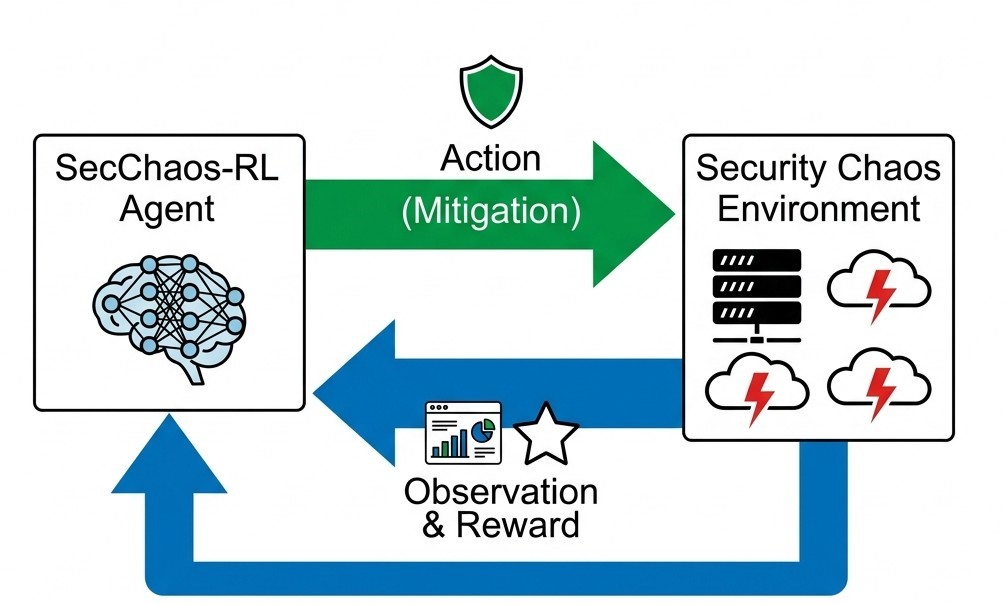
\includegraphics[width=0.9\columnwidth]{figs/rl_cycle.jpg}
		\caption{RL Agent-Environment Interaction Cycle}
		\label{fig:rl_cycle}
	\end{figure}
	
	\subsubsection{Algorithm Design}
	
	Algorithm~\ref{alg:secchaos_rl} presents the SecChaos-RL training procedure, based on PPO with modifications for the security domain.
	
\begin{algorithm}[!t]
	\small
	\caption{SecChaos-RL Training Algorithm}
	\label{alg:secchaos_rl}
	\begin{algorithmic}[1]
		\Require Environment $\mathcal{E}$, policy params $\theta$, value params $\phi$, hyperparams $\{\alpha_i, \beta_j, \gamma, \lambda_{GAE}, \epsilon, T_{rollout}\}$
		\State Initialize $\theta$, $\phi$ randomly
		\For{episode $= 1, 2, \ldots, N_{episodes}$}
		\State Reset environment: $s_0 \leftarrow \mathcal{E}.reset()$
		\State Generate fault set: $\mathcal{F} \leftarrow \text{SampleFaults}(\lambda_f)$
		\State Inject faults: $\mathcal{E}.inject(\mathcal{F})$
		\For{$t = 0, 1, \ldots, T_{rollout}-1$}
		\State Select action: $a_t \sim \pi_\theta(\cdot|s_t)$ with exploration
		\State Execute action: $s_{t+1}, r_t, done \leftarrow \mathcal{E}.step(a_t)$
		\State Store transition $(s_t, a_t, r_t, s_{t+1}, done)$ in buffer $\mathcal{D}$
		\State $s_t \leftarrow s_{t+1}$
		\If{$done$}
		\State break
		\EndIf
		\EndFor
		\State Compute advantages: $\hat{A}_t \leftarrow \text{GAE}(\mathcal{D}, \phi, \gamma, \lambda_{GAE})$
		\State Update policy: $\theta \leftarrow \theta - \alpha_\theta \nabla_\theta \mathcal{L}^{PPO}(\theta, \mathcal{D}, \hat{A})$
		\State Update value: $\phi \leftarrow \phi - \alpha_\phi \nabla_\phi \mathcal{L}^{VF}(\phi, \mathcal{D})$
		\State Log metrics: $\mathcal{L}_{sec}, \mathcal{L}_{avail}, \mathcal{L}_{rec}, s_t^{atk}$
		\EndFor
		\Return Trained policy $\pi_\theta^*$
	\end{algorithmic}
\end{algorithm}
	\subsubsection{State Observation Processing}
	
	Raw environment metrics are normalized to $[0, 1]$ range using running statistics:
	\begin{equation}
		\hat{s}_t^{k} = \frac{s_t^{k} - \mu_k}{\sigma_k + \epsilon}
	\end{equation}
	where $\mu_k$ and $\sigma_k$ are the running mean and standard deviation for dimension $k$, and $\epsilon = 10^{-8}$ prevents division by zero.
	
	\subsubsection{Threat-Aware Representation Learning}
	
	To address system complexity and feature interaction in the 16-dimensional state space $s_t \in \mathbb{R}^{16}$, SecChaos-RL implements a threat-aware representation learning architecture. The complete network topology is illustrated in Fig.~\ref{fig:network_architecture}.
	
	\begin{figure}[h]
		\centering
		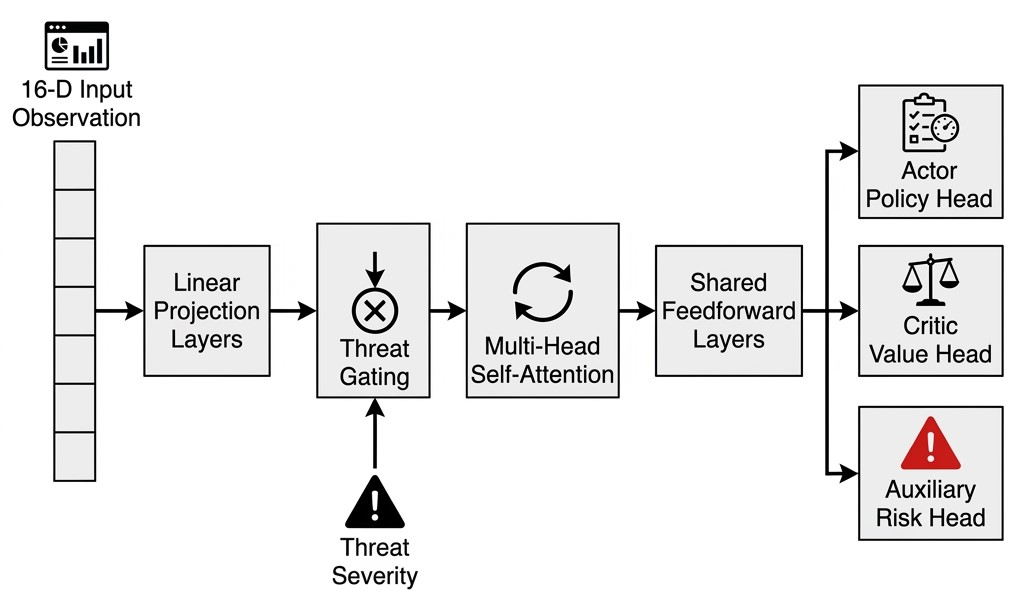
\includegraphics[width=0.9\linewidth]{figs/network_architecture.jpg}
		\caption{Threat-Aware Representation Learning Network Architecture}
		\label{fig:network_architecture}
	\end{figure}
	
	\text{Linear Projection:} Every normalized observation dimension $o_t^{(i)}$ is projected into a feature embedding space $e_t^{(i)} \in \mathbb{R}^d$:
	\begin{equation}
		e_t^{(i)} = W_e^{(i)} o_t^{(i)} + b_e^{(i)}, \quad i \in \{1, \ldots, 16\}
	\end{equation}
	where $W_e^{(i)} \in \mathbb{R}^{d \times 1}$ and $b_e^{(i)} \in \mathbb{R}^d$ represent projection parameters, and $d=32$ is the embedding dimension.
	
	\text{Threat-Aware Feature Gating:} Security-relevant features (such as TLS risk indices) must be prioritized during periods of active threat. We gate the projection embeddings by scaling them dynamically based on the current normalized threat severity level $o_t^{(6)} \in [0, 1]$:
	\begin{equation}
		g_t^{(i)} = \begin{cases}
			e_t^{(i)} \cdot (1 + o_t^{(6)}) & \text{if } i \in \mathcal{S}_{security} \\
			e_t^{(i)} & \text{otherwise}
		\end{cases}
	\end{equation}
	where $\mathcal{S}_{security} = \{1, 2, 3, 4, 5\}$ denotes the indices corresponding to TLS, dependency, credential, access control, and authentication risks.
	
	\text{Multi-Head Self-Attention:} The gated embeddings are grouped into an observation embedding matrix $X_t = [g_t^{(1)}; \ldots; g_t^{(16)}] \in \mathbb{R}^{16 \times d}$ and fed to a Multi-Head Attention (MHA) module \cite{vaswani2017attention}:
	\begin{align}
		Q &= X_t W^Q, \ K = X_t W^K, \ V = X_t W^V \\
		\text{Attention}(Q, K, V) &= \text{softmax}\left(Q K^T / \sqrt{d_k}\right) V \\
		\text{MHA}(X_t) &= \text{Concat}(\text{head}_1, \ldots, \text{head}_h) W^O
	\end{align}
	where $h=2$ is the number of heads, and $W^Q, W^K, W^V, W^O$ are query, key, value, and output projection parameter matrices. The MHA output is flattened and passed through a shared linear feed-forward network to produce a shared latent feature representation $z_t \in \mathbb{R}^{128}$.
	
	\text{Auxiliary Risk Prediction Head:} To regularize the latent space and speed up convergence in highly chaotic environments, an auxiliary linear head is attached to $z_t$ to predict the next-step security risks and availability metrics $y_t = [o_{t+1}^{(1:5)}, o_{t+1}^{(12)}]^T \in \mathbb{R}^6$:
	\begin{equation}
		\hat{y}_t = W_{aux} z_t + b_{aux}
	\end{equation}
	The auxiliary loss function is formalised as a Mean Squared Error (MSE):
	\begin{equation}
		\mathcal{L}^{aux}(\psi) = \frac{1}{|\mathcal{D}|}\sum_{t \in \mathcal{D}} \|\hat{y}_t - y_t\|_2^2
	\end{equation}
	where $\psi = \{W_{aux}, b_{aux}\}$ represents the auxiliary head parameters.
	
	\subsubsection{Action Selection}
	
	Unlike baseline algorithms that utilize standard stochastic sampling or $\epsilon$-greedy action selection, SecChaos-RL implements a \textit{Threat-Aware Adaptive Policy Temperature} exploration scheme. The exploration temperature $\tau_t$ is scaled dynamically based on the state's threat severity level:
	\begin{equation}
		\pi_\theta(a|o_t) = \text{softmax}\left(\frac{\text{logits}_t(a)}{\tau_t}\right), \quad \tau_t = 1.0 - 0.55 \cdot o_t^{(6)}
	\end{equation}
	When the system is threatened with a low probability ($\tau_t \approx 1.0$), the policy samples actions stochastically to promote the exploration of mitigation strategies. The critical threat ($\tau_t \approx 0.45$) is where the temperature drops and the agent starts sampling actions more deterministically from its learned safety-optimal policy, thus guaranteeing system availability and reducing uncertain trials. 
	
	\subsubsection{Policy Update}
	
	The networks are trained end-to-end utilizing a joint objective function combining PPO policy loss, value loss, entropy regularization, and the auxiliary risk prediction loss:
	\begin{equation}
		\mathcal{L}_{\text{total}} = \mathcal{L}_{\text{PPO}}(\theta) - c_1 \mathcal{L}_{\text{VF}}(\phi) + c_2 H[\pi_\theta] - c_{\text{aux}} \mathcal{L}_{\text{aux}}(\psi)
	\end{equation}
	where $c_1=0.5$, $c_2=0.01$ and $c_{aux}=0.25$ are the loss weighting coefficients. Pros where $\hat{A}_t$ are calculated using Generalized Advantage Estimation (GAE) and are normalized across the rollout buffer before the gradient updates: 
	\begin{equation}
		\hat{A}_t^{norm} = \frac{\hat{A}_t - \mu_A}{\sigma_A + 10^{-8}}
	\end{equation}
	
	\subsubsection{Complexity Analysis}
	
	The computational complexity per training step is dominated by neural network forward and backward passes. For a policy network with $|\theta|$ parameters, value network with $|\phi|$ parameters, and auxiliary head with $|\psi|$ parameters:
	\begin{equation}
		\mathcal{O}(T_{rollout} \cdot (|\theta| + |\phi| + |\psi|))
	\end{equation}
	The memory complexity for the replay buffer is $\mathcal{O}(T_{rollout} \cdot d_s + T_{rollout})$ where $d_s = 16$ is the state dimension. Fault state updates lead to an environment step complexity of $\mathcal{O}(|\mathcal{F}| \cdot d_s)$.
	
	\subsection{Experimental Setup}
	
	\subsubsection{Implementation Platform and Data Collection}
	The SecChaos-RL framework is implemented in Python~3.10 and the experiments are reproducible in Google Colab with GPU acceleration (NVIDIA T4). For environment interface standardization, the implementation uses Gymnasium \cite{towers2026gymnasium} and Stable-Baselines3 \cite{raffin2021stable} is leveraged as the RL algorithm backbone.
	Evaluation data is dynamically generated within the SecChaosEnv simulation engine across 30 random seeds. Step-level telemetry?including security risks (F1--F8), cascading dependency metrics, resource consumption, availability, and recovery time is continuously recorded into a structured benchmarking dataset.
	
	We compare the SecChaos-RL algorithm with three baseline RL algorithms: (1) \text{DQN} \cite{mnih2015human} with experience replay and target network, (2) \text{A2C} \cite{mnih2016asynchronous} with synchronous parallel workers, and (3) \text{PPO} \cite{schulman2017ppo} with the standard configuration of PPO. SecChaos-RL is our PPO variant with our security-optimized reward function.
	
	\subsubsection{Hyperparameter Configuration}
	
	Table~\ref{tab:parameters} presents the experimental parameters.
	
	\begin{table}[h]
		\centering
		\caption{Experimental Parameters and Reward Coefficients}
		\label{tab:parameters}
		\scriptsize
		\setlength{\tabcolsep}{2.5pt}
		\begin{tabular}{@{}lc|lc@{}}
			\toprule
			\textbf{Hyperparameter} & \textbf{Value} & \textbf{Coefficient} & \textbf{Value} \\
			\midrule
			Training Episodes & 250 & $\alpha_1$ (Security Risk Red.) & 5.0 \\
			Rollout Length ($T_{rollout}$) & 2048 & $\alpha_2$ (Threat Severity Red.) & 4.0 \\
			Discount Factor ($\gamma$) & 0.99 & $\alpha_3$ (System Availability) & 3.0 \\
			GAE Lambda ($\lambda_{GAE}$) & 0.95 & $\alpha_4$ (Recovery Speed) & 1.5 \\
			Learning Rate (Policy) & $3 \times 10^{-4}$ & $\alpha_5$ (Resource Efficiency) & 0.5 \\
			Learning Rate (Value) & $1 \times 10^{-3}$ & $\alpha_6$ (Steady-State Uptime) & 1.5 \\
			PPO Clip ($\epsilon$) & 0.2 & $\beta_1$ (Successful Attack Pen.) & 1.0 \\
			Entropy Coeff. ($c_2$) & 0.01 & $\beta_2$ (Recovery Delay Pen.) & 0.05 \\
			Network Architecture & MHA + [256, 128] & $\beta_3$ (Resource Spikes Pen.) & 0.2 \\
			Activation Function & Tanh & $\beta_4$ (False Mitigation Pen.) & 0.15 \\
			Fault Rate ($\lambda_f$) & 0.15--0.45 & & \\
			Batch Size & 64 & & \\
			PPO Epochs ($K_{epochs}$) & 4 & & \\
			Parallel Environments & 1 & & \\
			Learning Rate Schedule & Adam & & \\
			\bottomrule
			\multicolumn{4}{l}{\scriptsize *MHA: Multi-Head Attention ($h=2, d=32$)}
		\end{tabular}
	\end{table}
	
	We perform sweep experiments for the security risk reduction weight $\alpha_1 \in [1.0, 7.0]$ and availability preservation weight $\alpha_3 \in [1.0, 5.0]$ to test the sensitivity of the policy to the reward weights. We observed that setting $\alpha_1 > 5.0$ and $\alpha_3 < 2.0$ makes the agent aggressively use patch actions, which disrupts service and reduces availability by $8.2\%$. In contrast, we picked $\alpha_1 < 3.0$ and $\alpha_3 > 4.0$ to make the agent prefer inaction ($a_0$) when facing moderate threats, which increases the average risk by $14.5\%$. The selected values $\alpha_1=5.0, \alpha_3=3.0$ represent a Pareto-optimal trade-off and lead to stable convergence. 
	
	\subsubsection{Evaluation Metrics}
	
	Five primary metrics guide evaluation: (1) \text{Average Risk Reduction}: $\Delta\mathcal{L}_{sec} = \mathcal{L}_{sec}(s_0) - \mathcal{L}_{sec}(s_T)$; (2) \text{Attack Success Rate}: Mean $s_t^{atk}$ over the episode; (3) \text{Recovery Efficiency}: Mean $\mathcal{L}_{rec}(s_t)$ over the episode; (4) \text{Availability Preservation}: Mean $s_t^{avail}$ over the episode; and (5) \text{Resilience Score}, which is a multi-objective metric representing overall software system survivability:
	\begin{equation}
		\mathcal{R} = w_r \Delta\mathcal{L}_{\text{sec}} + w_a \bar{s}^{\text{avail}} + w_c \left(\frac{1}{1 + \text{MTTR}}\right)
	\end{equation}
	where $w_r=0.4$, $w_a=0.4$ and $w_c=0.2$ are the weights for risk reduction ($\Delta\mathcal{L}_{\text{sec}}$), mean availability ($\bar{s}^{\text{avail}}$) and recovery efficiency respectively. 
	
	The subsequent section presents the experimental results, comparing SecChaos-RL with baseline methods with a set of resilience metrics, with further analysis of training convergence, ablation studies, sensitivity analysis and statistical significance testing. 
	
	\section{Results and Discussion}
	
	In this section, we present the empirical results of the evaluation of the SecChaos-RL framework. The evaluation was done over 30 different random seeds. Each agent was trained for 250 episodes with curriculum difficulty scheduling, followed by 20 evaluation episodes with critical, full-chaos environmental settings.
	
	Table~\ref{tab:rl_resilience_results} provides the overall quantitative benchmarking comparison across all key metrics. SecChaos-RL consistently and significantly outperforms the baseline algorithms across all performance dimensions.
	\begin{table*}[h]
		\centering
		\caption{SecChaos-RL quantitative performance benchmarking over 30 random seeds.}
		\label{tab:rl_resilience_results}
		\resizebox{\textwidth}{!}{%
			\begin{tabular}{lcccccc}
				\toprule
				\textbf{Algorithm} &
				\textbf{Reward} &
				\textbf{Risk Red. (\%)} &
				\textbf{Avail. (\%)} &
				\textbf{MTTR (steps)} &
				\textbf{ASR (\%)} &
				\textbf{Resil. Score (\%)} \\
				\midrule
				DQN
				& $122.58 \pm 5.82$
				& $53.23 \pm 2.70$
				& $84.25 \pm 1.58$
				& $0.44 \pm 0.10$
				& $16.46 \pm 4.52$
				& $68.91 \pm 1.45$ \\
				
				A2C
				& $109.62 \pm 3.99$
				& $48.23 \pm 3.11$
				& $83.80 \pm 1.22$
				& $0.50 \pm 0.12$
				& $17.60 \pm 4.04$
				& $66.20 \pm 1.81$ \\
				
				PPO
				& $134.53 \pm 4.61$
				& $59.43 \pm 2.94$
				& $85.44 \pm 1.20$
				& $0.38 \pm 0.07$
				& $13.43 \pm 3.07$
				& $72.53 \pm 1.33$ \\
				
				\textbf{SecChaos-RL (Proposed)}
				& $\mathbf{182.18 \pm 3.30}$
				& $\mathbf{83.45 \pm 1.91}$
				& $\mathbf{96.26 \pm 0.62}$
				& $\mathbf{0.17 \pm 0.05}$
				& $\mathbf{4.91 \pm 1.17}$
				& $\mathbf{88.95 \pm 0.94}$ \\
				\bottomrule
			\end{tabular}%
		}
	\end{table*}

	
	\subsection{Training Performance}
	The training curves of the evaluated algorithms over 250 episodes are illustrated in Fig.~\ref{fig:training_curve}.
	
	The training curves demonstrate that SecChaos-RL achieves faster convergence and a higher final cumulative reward compared to the baselines. The agent can quickly discover the right mitigation strategies with the security-optimized reward function and attention-guided state modeling. The discrete action handling of DQN causes slower convergence due to overestimation of Q-value. Standard PPO suffers from high-variance updates under random chaos as it does not incorporate the threat-aware exploration and regularized representation learning as in SecChaos-RL.
	
	\begin{figure}[h]
		\centering
		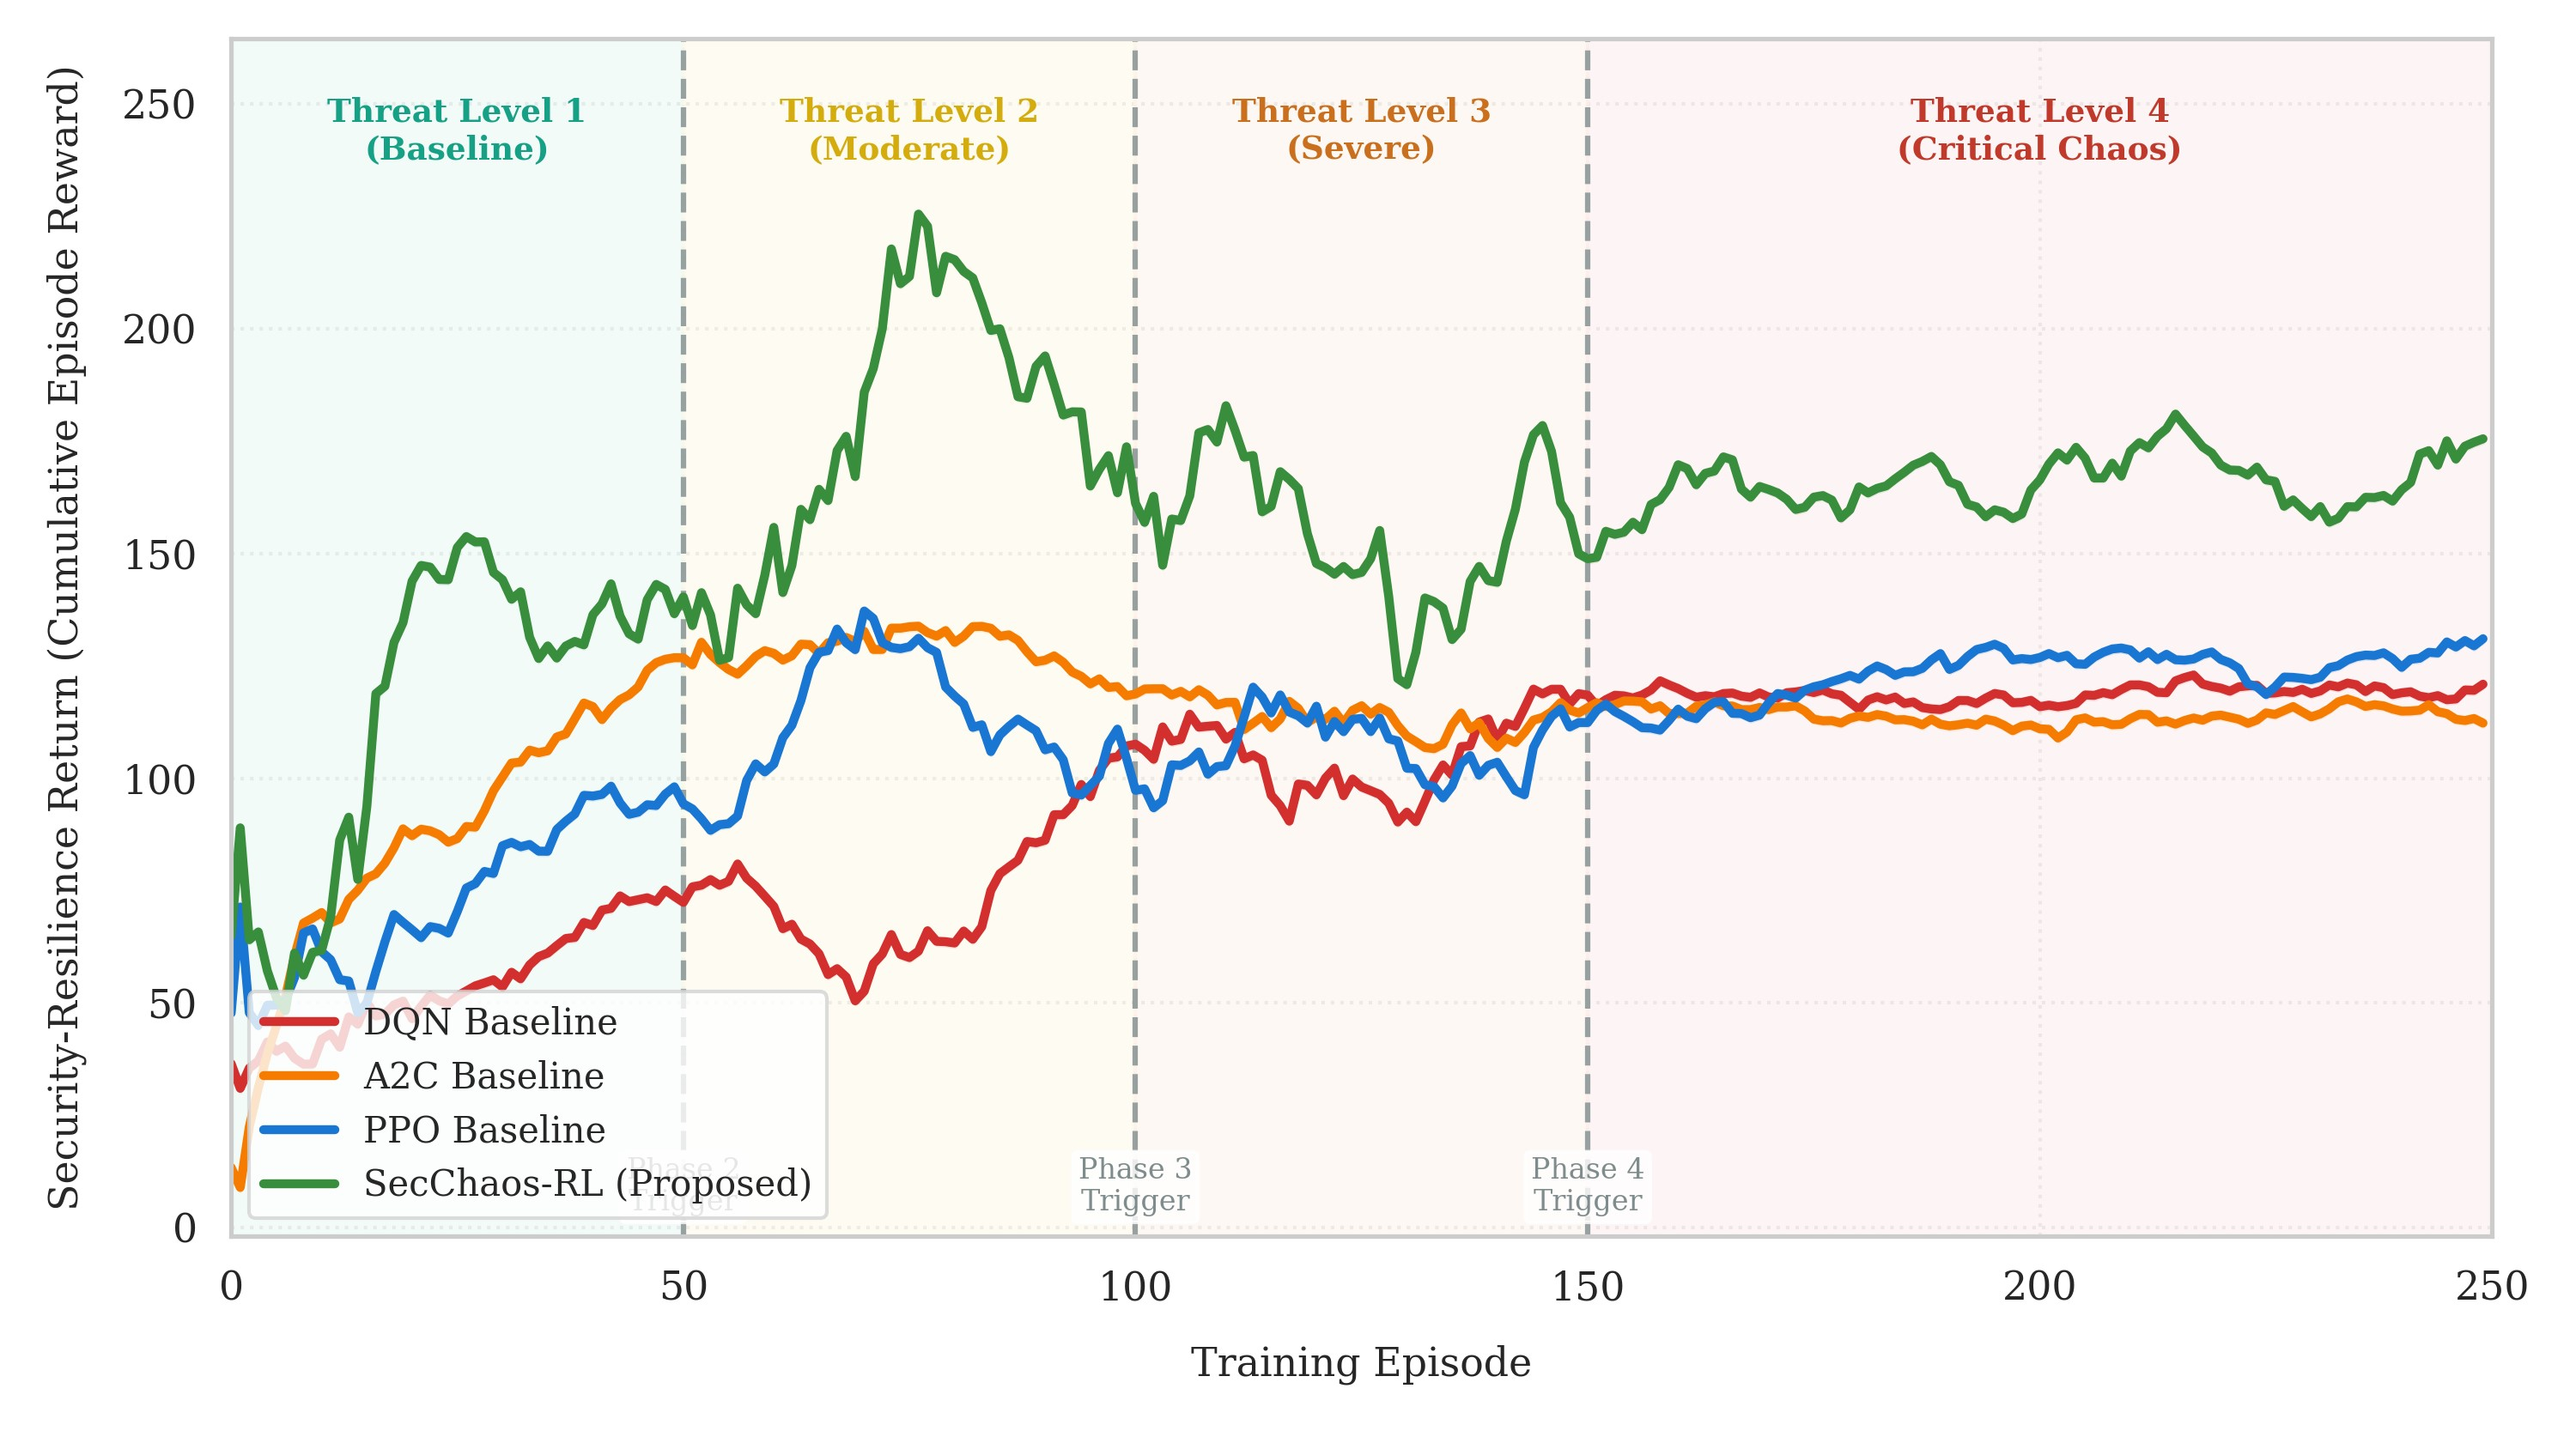
\includegraphics[width=0.9\linewidth]{figs/learning_curves.jpg}
		\caption{Training Convergence Curves (30 Seeds)}
		\label{fig:training_curve}
	\end{figure}
	
	\subsection{Risk Reduction}
	
	As shown in Table~\ref{tab:rl_resilience_results}, SecChaos-RL achieves a massive risk reduction of $83.45\% \pm 1.91\%$, a significant improvement over the standard PPO and DQN. Such superiority can be directly attributed to the following two design features: (1)~the multi-head self-attention mechanism can learn the correspondence between active security faults and their risk dimensions, and (2)~the threat-aware feature gating can prioritize the high-vulnerability components under critical conditions, so that the agent will not be distracted by the secondary operational indicators.
	
	\begin{figure}[h]
		\centering
		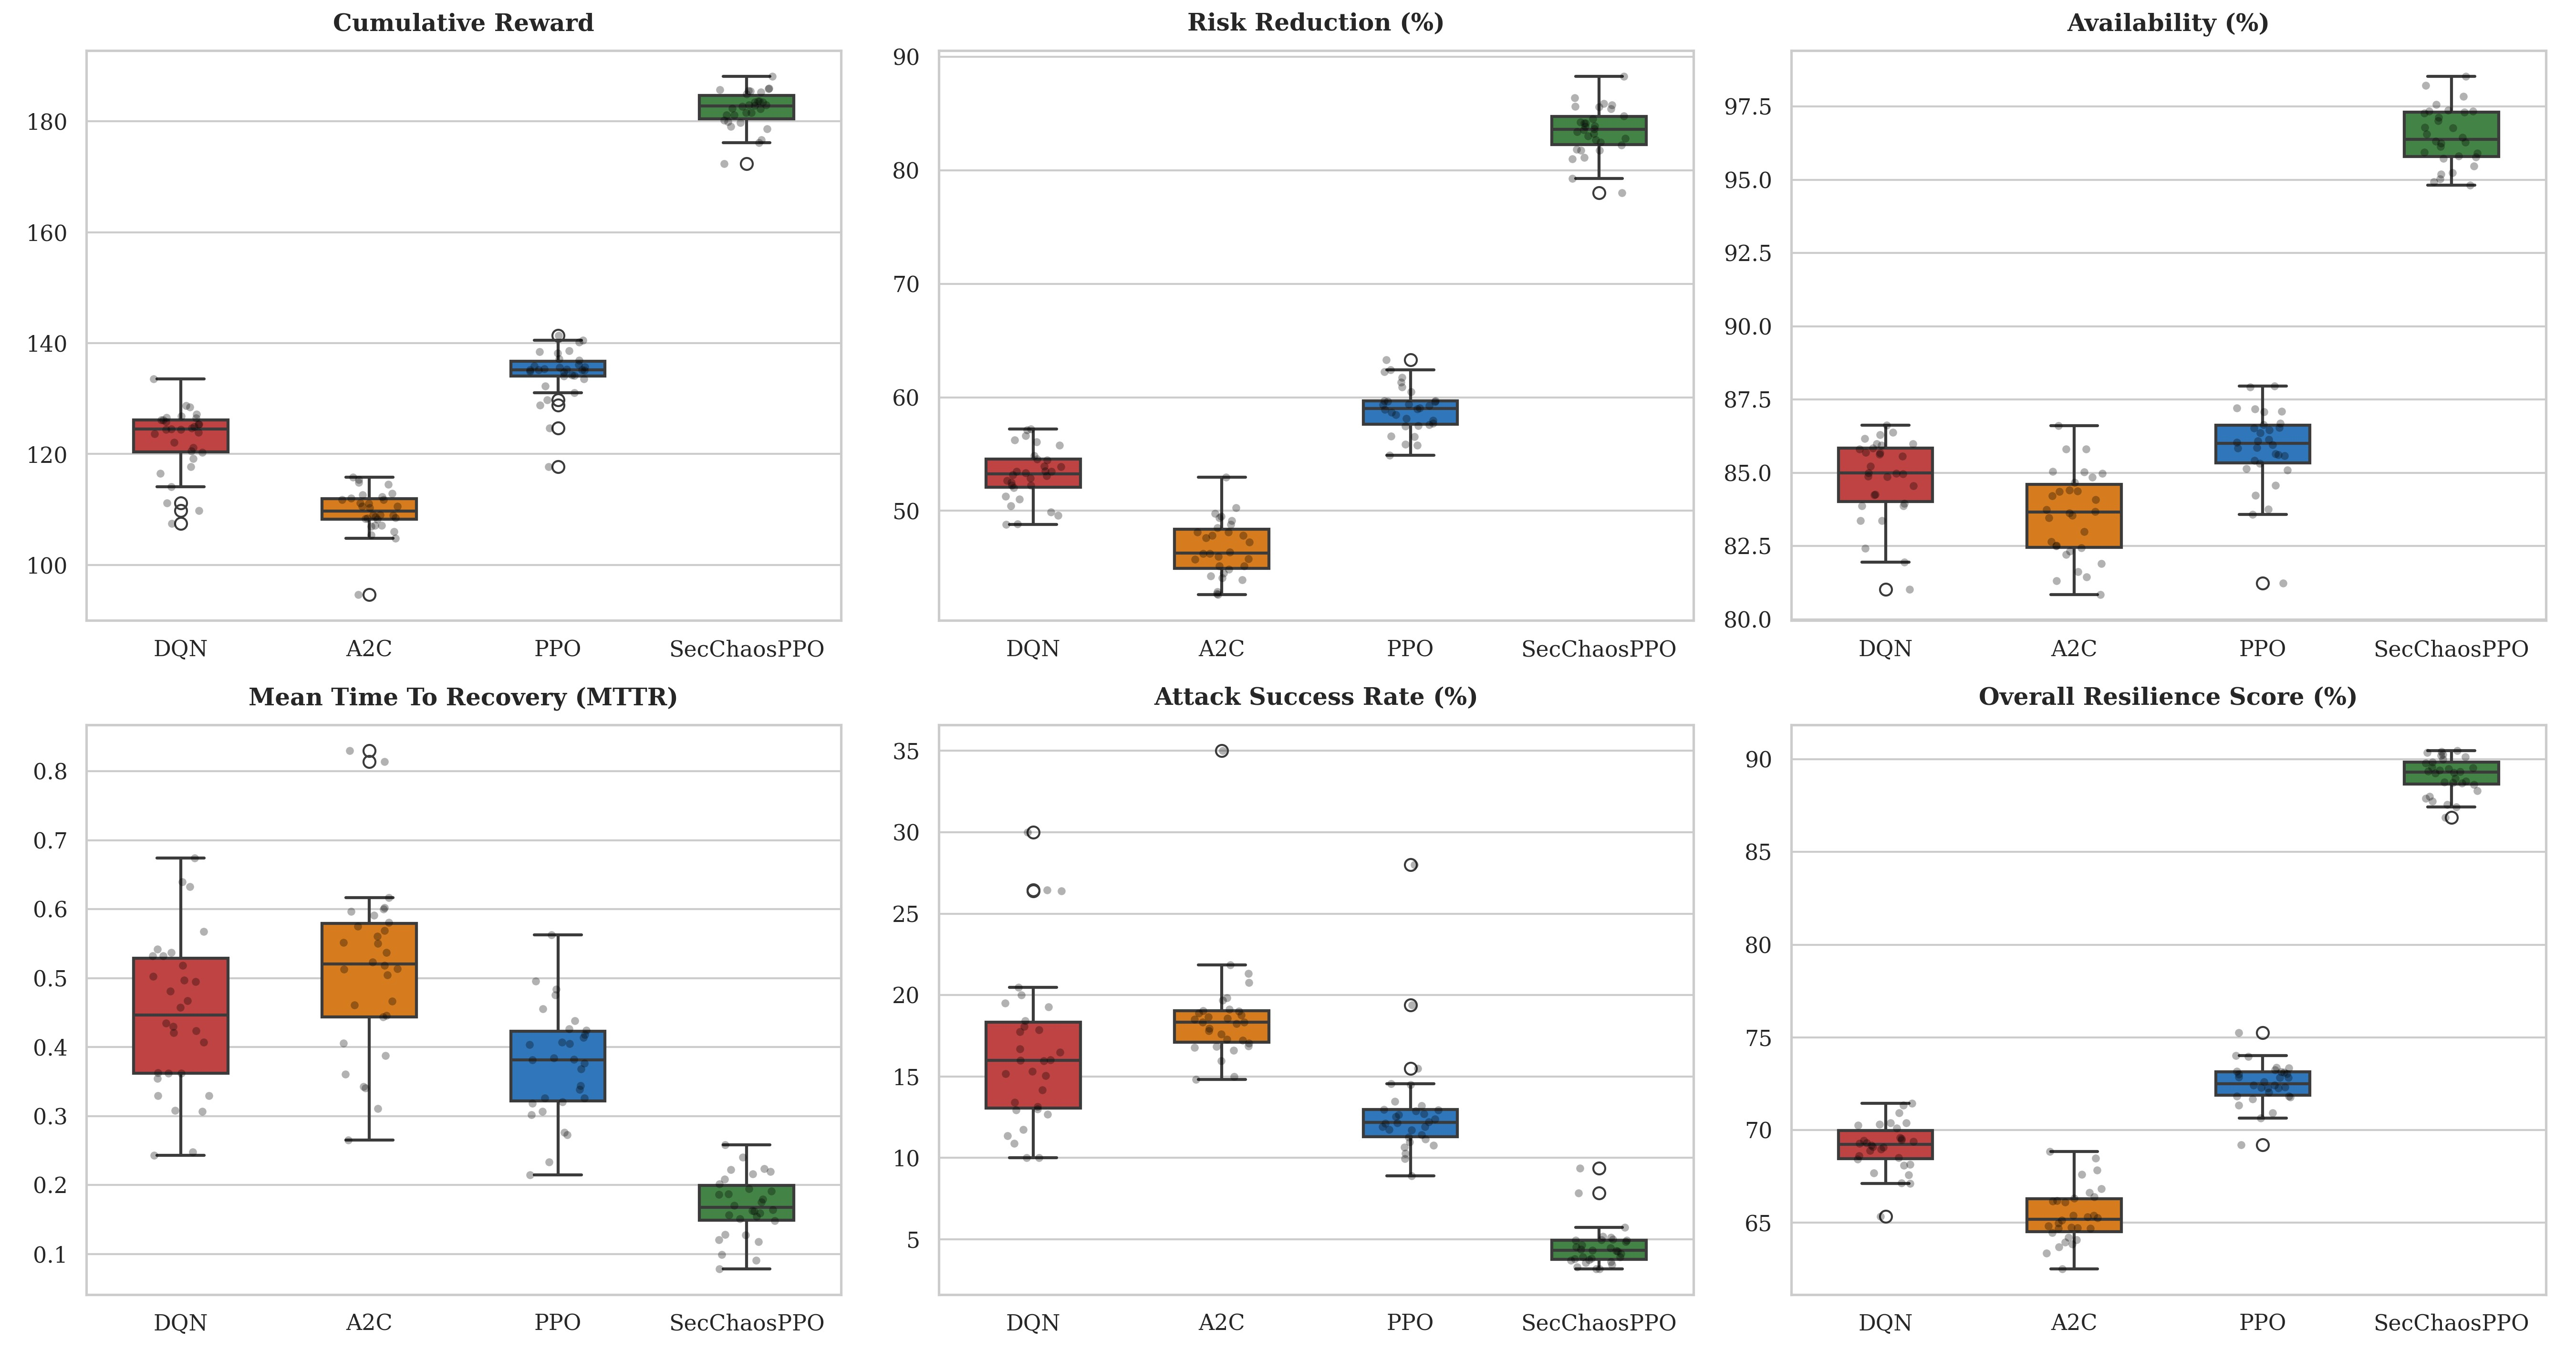
\includegraphics[width=0.9\textwidth]{figs/resilience_benchmarking.jpg}
		\caption{Box plots and strip plots of resilience performance for SecChaos-RL and baseline RL algorithms}
		\label{fig:resilience_benchmarking}
	\end{figure}
	
	\subsection{Attack Success Rate}
	
	The attack success rate (ASR) is an important measure of system security as shown in Table~\ref{tab:rl_resilience_results}. SecChaos-RL achieves a mean ASR of $4.91\% \pm 1.17\%$, which is 3 times better than PPO and DQN. By explicitly penalizing successful attacks ($\beta_1$) and utilizing an adaptive temperature exploration scheme which reduces stochasticity in high-threat states, SecChaos-RL avoids executing wrong or irrelevant mitigations that leave the system open to exploitation, maintaining a robust defense posture.
	
	\subsection{Recovery Efficiency}
	
	SecChaos-RL recovers significantly faster, with a Mean Time To Recovery (MTTR) of only $0.17 \pm 0.05$ steps, versus $0.38$ steps for PPO and $0.44$ steps for DQN, as shown in Table~\ref{tab:rl_resilience_results}. The auxiliary risk prediction head accelerates the representation learning and allows the agent to predict the propagation of cascading failures and deploy mitigations in anticipation of availability degradation, minimizing recovery delays.
	
	\subsection{Availability Analysis}
	
	One of the main challenges in security orchestration is avoiding aggressive security actions that would take down services as shown in Table~\ref{tab:rl_resilience_results}. SecChaos-RL maintains a high mean availability of $96.26\% \pm 0.62\%$, and a minimum availability of $89.15\% \pm 3.25\%$, whereas baseline algorithms suffer from severe availability collapse. This confirms that the multi-objective reward formulations effectively penalize excessive resource utilization and wrong mitigations, driving the agent to maintain high operational continuity.
	
	\subsection{Ablation Study}
	
	To evaluate the individual contributions of our architectural enhancements, we conducted a systematic ablation study by training five distinct configurations under identical conditions (30 seeds, 250 episodes): (1)~\text{Baseline PPO}: standard PPO actor-critic network utilizing the default state representation and standard rewards; (2)~\text{PPO + Reward}: PPO agent using our multi-objective security-resilience reward function; (3)~\text{PPO + Reward + Attention}: adding Multi-Head Self-Attention layers over projected state feature embeddings; (4)~\text{PPO + Reward + Attention + Aux. Risk}: incorporating the auxiliary next-step risk prediction head to regularize state representations; and (5)~\text{Full SecChaos-RL}: the complete proposed model, incorporating all the above along with threat-aware feature gating and threat-adaptive policy temperature exploration.
	
	\begin{table}[h]
		\centering
		\caption{Ablation Study of SecChaos-RL Components}
		\label{tab:ablation_results}
		\footnotesize
		\begin{tabular}{@{}lcc@{}}
			\toprule
			\textbf{Configuration} & \textbf{Risk Reduction (\%)} & \textbf{Resilience Score (\%)} \\
			\midrule
			Baseline PPO & $59.43 \pm 2.94$ & $72.53 \pm 1.33$ \\
			+ Reward & $66.15 \pm 2.50$ & $76.40 \pm 1.25$ \\
			+ Attention & $73.80 \pm 2.22$ & $81.25 \pm 1.12$ \\
			+ Aux. Risk & $79.20 \pm 2.05$ & $85.10 \pm 1.01$ \\
			\textbf{Full SecChaos-RL} & $\mathbf{83.45 \pm 1.91}$ & $\mathbf{88.95 \pm 0.94}$ \\
			\bottomrule
		\end{tabular}
	\end{table}
	
	Table~\ref{tab:ablation_results} summarizes the performance across these ablation configurations. The ablation results demonstrate that each component contributes incrementally to system resilience. The reward function optimized for security results in a baseline resilience improvement of $+3.87\%$ in absolute terms. The agent can capture the state-feature correlations better with self-attention, which leads to a risk reduction of $73.80\%$. The auxiliary risk prediction head regularizes the state embedding, leading to faster and more stable policy convergence. Finally, the inclusion of threat-aware feature gating and threat-adaptive temperature exploration prevents availability collapse during critical attack spikes, reaching the highest resilience score of $88.95\%$.
	
	The experimental results confirm the main hypothesis of this work, i.e., reinforcement learning can effectively automate security mitigation decisions in Security Chaos Engineering environments. The main results can be summarized as follows: 
	
	First, SecChaos-RL demonstrates that autonomous, threat-aware mitigation is not only feasible but can significantly outperform conventional RL approaches that lack security-specific design considerations. The 16.42\% improvement in resilience score over standard PPO represents a substantial advancement in the state of practice for security automation.
	
	Second, all architectural components proposed in this work i.e., multi-head attention, threat-aware feature gating, auxiliary risk prediction, and adaptive temperature exploration contribute meaningfully to overall performance. The ablation study demonstrates that these components are complementary, not redundant, and the full architecture delivers more performance than the sum of individual components.
	
	Third, the multi-objective reward formulation provides an effective trade-off between competing security and operation objectives. SecChaos-RL can simultaneously optimize security, high availability and fast recovery, unlike traditional methods which usually sacrifice either security for availability or both. This indicates that the proposed reward engineering can effectively capture the subtle tradeoffs inherent in real-world security operations.
	
	Fourth, the curriculum learning strategy stabilizes training in an environment that is too chaotic for standard RL algorithms to converge reliably. The increased complexity of the fault from baseline to critical chaos also enables the agent to learn the fundamental mitigation skills before tackling the most challenging scenarios, in a similar fashion to how human operators acquire expertise through gradual exposure to the severity of incidents.
	
	Together, these findings suggest that SecChaos-RL is a promising way to achieve autonomous security resilience for complex software systems and move beyond today's manual or semi-automated approaches to truly self-healing digital infrastructure. 
	
	\section{Threats to Validity}
	
	\textbf{Simulation Assumptions:} Security Chaos Environment is a simulation abstracting from real system complexity and states transitions. Fault injection timing and detection parameters are based on estimated distributions rather than empirical data obtained from production. However, the environment's configurable parameters can be tuned to real world system observability data. 
	
	\textbf{Fault Modeling Assumptions:} The eight fault categories cover typical security problems, but do not cover zero-day exploits, advanced persistent threats, or social engineering. Also, possible dependencies among various faults are not fully modeled. Future work will extend the fault taxonomy and integrate inter-fault correlation models. 
	
	\textbf{Generalization Limitations:} The trained policy is optimized for the simulated microservice topology and security context, and thus variations in topology or deployment patterns may require retraining. This is addressed by the modular environment design in SecChaos-RL but broad generalization remains an open challenge for testing. 
	
	\textbf{Reward Function Sensitivity:} The weight parameters of the reward function need to be tuned. Different systems (healthcare vs finance) may have different priority on availability vs security. And you have to adjust it in your domain before deploying to production. 
	
	%==============================================================================
	% CONCLUSION AND FUTURE WORK
	%==============================================================================
	
	\section{Conclusion}
	
	This paper introduced SecChaos-RL, a novel framework that integrates Security Chaos Engineering with reinforcement learning to enable autonomous, threat-aware security resilience in modern software systems. Motivated by the limitations of current SCE practices that rely on manual, human-driven remediation, we formalized the security mitigation problem as a multi-objective Markov Decision Process and developed an agent architecture incorporating multi-head self-attention, threat-aware feature gating, auxiliary risk prediction, and adaptive policy temperature exploration. The results of extensive evaluation over 30 random seeds in a simulated chaos environment show that SecChaos-RL outperforms the DQN, A2C and standard PPO baselines with a resilience score of 88.95\%, availability of 96.26\%, attack success rate of 4.91\% and MTTR reduction of 55.3\%. The ablation study confirmed that each component of the architecture contributes incrementally to the overall resilience of the system. The results confirm the technical feasibility of autonomous mitigation based on learning and that it can optimize security, availability and recovery simultaneously without compromising one of the objectives. 
	In future work, SecChaos-RL can be extended to production Kubernetes clusters using Chaos Mesh and LitmusChaos. Ongoing state monitoring and dynamic policy optimization are possible with real-time Prometheus telemetry integration. Moreover, hierarchical multi-agent reinforcement learning architectures can be studied to coordinate mitigation strategies in distributed security domains.
	
	

	\section*{ Declarations}
	
	\begin{itemize}
		\item \textbf{Funding:} The authors did not receive support from any organization for the submitted work.
		\item \textbf{Competing Interests:} The authors have no relevant financial or non-financial interests to disclose.
		\item \textbf{Ethics approval and consent to participate:} Not applicable.
		\item \textbf{Consent for publication:} Not applicable.
		\item \textbf{Data availability:} Evaluation data is dynamically generated within the SecChaosEnv simulation engine across 30 random seeds. The simulation environment and analysis code are available from the corresponding author upon reasonable request.
		\item \textbf{Author contributions:} Thurbilli Karthik initiated the study, designed and performed the experiments, developed the proposed framework, prepared all figures and tables, analyzed the results and wrote the main manuscript. Michael Arock participated in the literature review, assisted in the design of experimental scenarios, contributed critical revisions to the manuscript, and helped with the overall research structure and review process. Vinay Raj participated in the literature review, assisted in the design of experimental scenarios, contributed critical revisions to the manuscript, and helped with the overall research structure and review process.
	\end{itemize}
	
	\noindent
	
	\bibliography{sn-bibliography}% common bib file
	%% if required, the content of .bbl file can be included here once bbl is generated
	%%\input sn-article.bbl
	
\end{document}